\chapter{Results}
The final result of the project is a functional Android application that transforms the educational activity of the \textit{Jardín de los Sentidos} into a cooperative, geolocated serious game. The application allows players to create a multiplayer session, join it using a code and take part in a shared experience in which the group explores the real garden and completes missions linked to its sensory areas.

The application includes the main systems required to support the intended experience. It integrates geolocation so that the player’s real position can be used inside the game, a map scene that acts as the central navigation space, a cooperative multiplayer structure that keeps the session synchronised between devices, and a set of missions connected to the senses represented in the garden. The game also includes feedback after each mission and a final screen showing the group name, the participants and the score achieved during the session.

From a gameplay perspective, the result is a complete playable flow, as you can see Figures \ref{fig:q1}, \ref{fig:q2}, \ref{fig:q3}, \ref{fig:q4}, \ref{fig:dialogue} and \ref{fig:end}. Players can start a session, access the map, move through the garden, activate missions, solve them cooperatively and obtain a final result. The experience is structured around exploration, observation, communication and group decision-making, maintaining the relationship with the physical environment throughout the game.

\begin{figure}[h]
    \begin{multicols}{2} % Inicio de las dos columnas
        \begin{center}
            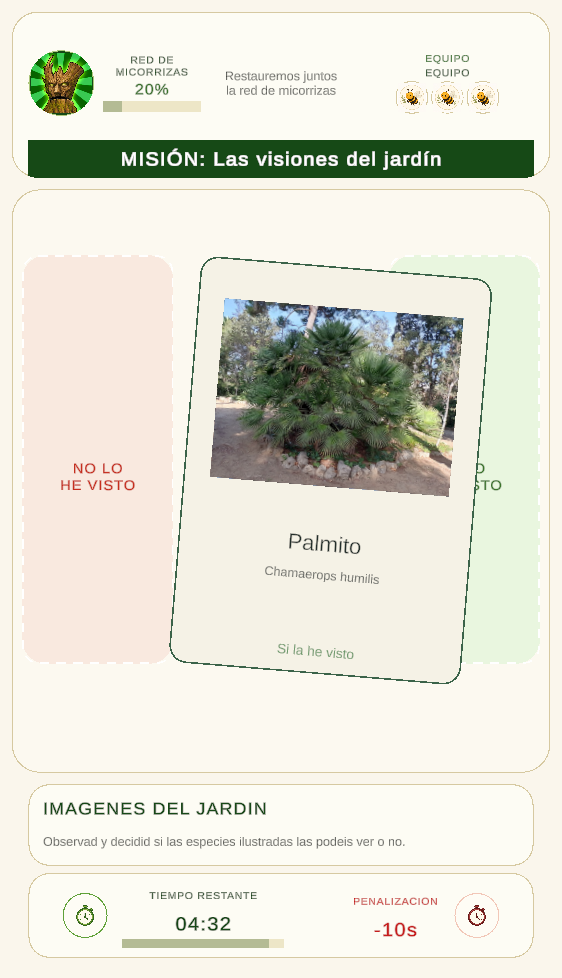
\includegraphics[width=0.5\textwidth]{img/ingame/quest1siVisto.png}
            \caption{Quest in the Garden of Sight area}
            \label{fig:q1}
        \end{center}
        
        \columnbreak
        
        \begin{center}
            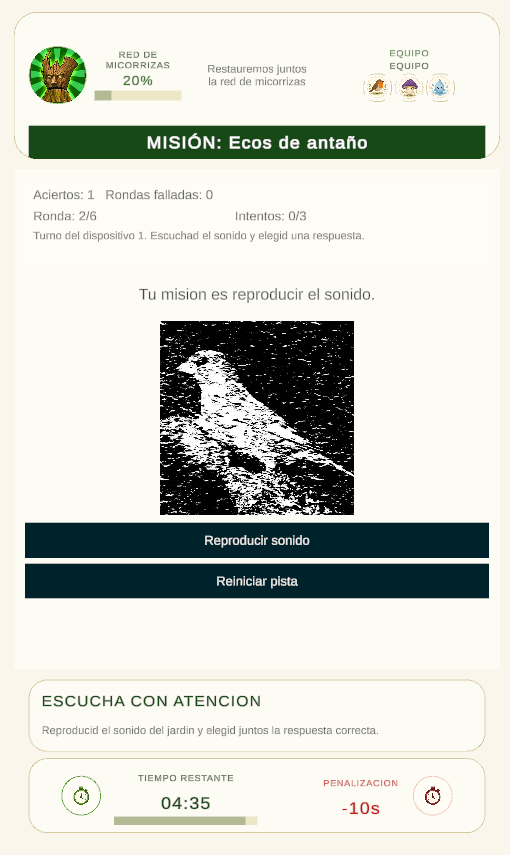
\includegraphics[width=0.5\textwidth]{img/ingame/quest2audio.png}
            \caption{Quest in the Garden of Hearing area}
            \label{fig:q2}
        \end{center}
    \end{multicols} % Fin de las dos columnas
\end{figure}

\begin{figure}[h]
    \begin{multicols}{2} % Inicio de las dos columnas
        \begin{center}
            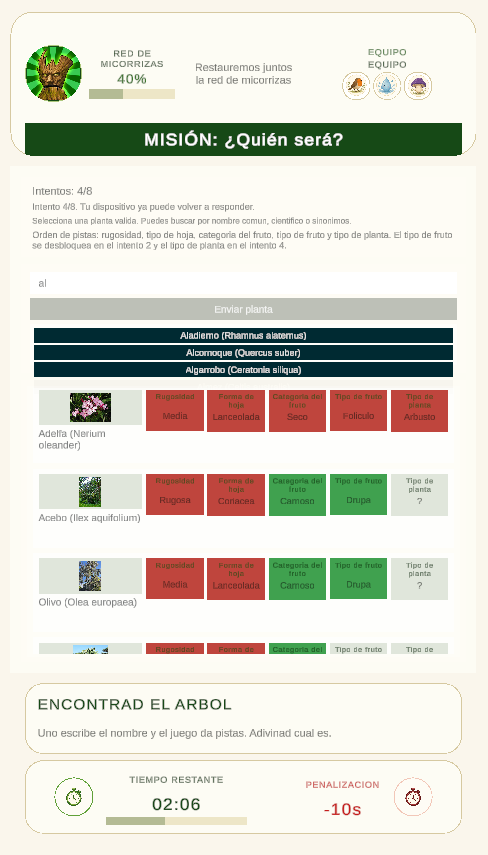
\includegraphics[width=0.5\textwidth]{img/ingame/quest3.png}
            \caption{Quest in the Garden of Touch area}
            \label{fig:q3}
        \end{center}
        
        \columnbreak
        
        \begin{center}
            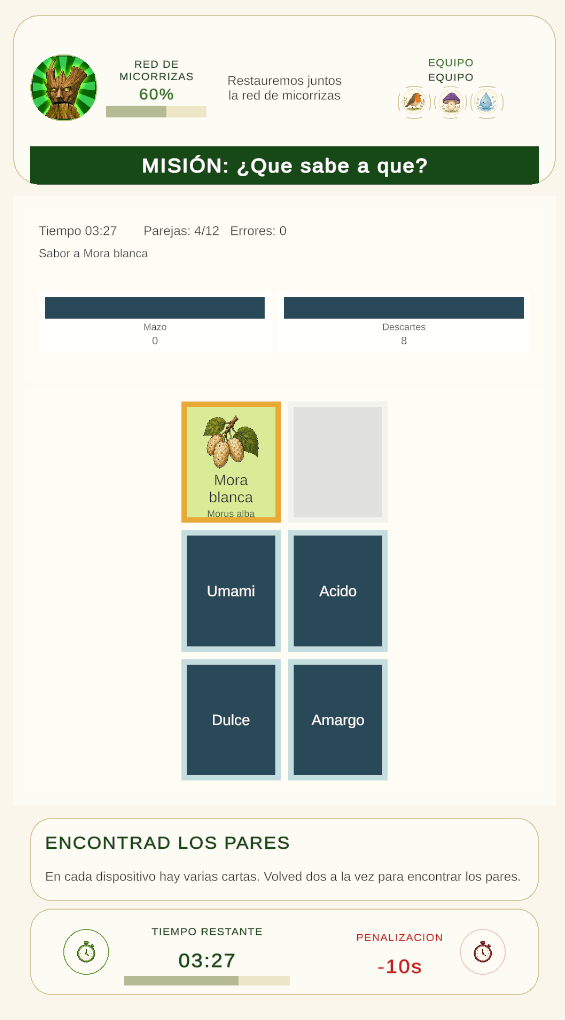
\includegraphics[width=0.5\textwidth]{img/ingame/quest4.png}
            \caption{Quest in the Garden of Taste area}
            \label{fig:q4}
        \end{center}
    \end{multicols} % Fin de las dos columnas
\end{figure}

\begin{figure}[h]
    \begin{multicols}{2} % Inicio de las dos columnas
        \begin{center}
            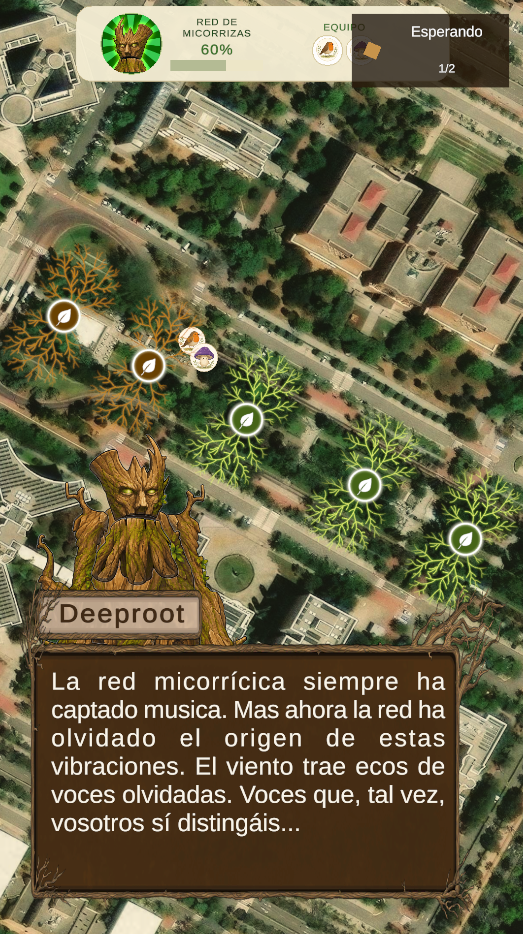
\includegraphics[width=0.5\textwidth]{img/ingame/Dialogue2.png}
            \caption{The dialogues with Deeproot, the companion and narrative guide in this story}
            \label{fig:dialogue}
        \end{center}
        
        \columnbreak
        
        \begin{center}
            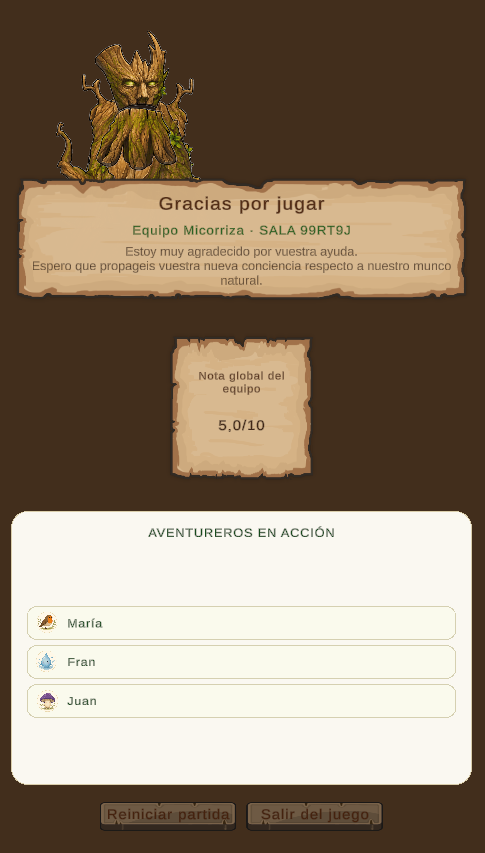
\includegraphics[width=0.5\textwidth]{img/ingame/end.png}
            \caption{End of the game: display the team's score and its members}
            \label{fig:end}
        \end{center}
    \end{multicols} % Fin de las dos columnas
\end{figure}

From an educational perspective, the application provides the lecturers with a digital tool that can be used to support the teaching session related to the \textit{Jardín de los Sentidos}. The final score and the group result can be used as part of the activity carried out in class, allowing the teachers to assess participation and performance during the session. In this sense, the project has produced a usable prototype that can be incorporated into the educational context for which it was designed.






% \chapter{Results}

% The project resulted in a functional Android prototype that transforms the educational activity of the \textit{Jardín de los Sentidos} into a cooperative, geolocated serious game. Players can create a multiplayer session, join it using a code, explore the garden and complete missions linked to its sensory areas.

% The prototype integrates a cooperative lobby, synchronised session state, GPS-based player positioning, an ArcGIS map scene, spatial mission activation, five cooperative mini-games, mission feedback and a final group summary.

% \section{Final prototype}

% The final build supports a complete playable flow. Players start a session, access the map, move through the garden, activate missions, solve them cooperatively and receive a final result. The experience is based on exploration, observation, communication and group decision-making.

% The five implemented missions are:

% \begin{itemize}
%     \item \textbf{Garden of Sight}: visual recognition of plant species through a card-swiping mechanic.
%     \item \textbf{Garden of Hearing}: cooperative sound identification with distributed answers between devices.
%     \item \textbf{Garden of Touch}: progressive deduction of plant species through successive clues.
%     \item \textbf{Garden of Taste}: cooperative memory game based on plants and fruits.
%     \item \textbf{Garden of Smell}: classification of plant cards according to their uses.
% \end{itemize}

% Deeproot provides narrative continuity between missions and frames progression as the restoration of the garden's mycorrhizal network. This gives the mini-games a shared purpose within the same experience.

% \section{Implemented systems}

% The main implemented systems are:

% \begin{itemize}
%     \item \textbf{Cooperative connection}: players can create or join a session through a room code.
%     \item \textbf{Shared session state}: the game synchronises the current phase, active mission and progression between devices.
%     \item \textbf{Geolocation service}: Android devices provide GPS readings used to represent players in the map scene.
%     \item \textbf{Map integration}: ArcGIS represents the physical space of the garden and places player markers.
%     \item \textbf{Mission activation}: sensory areas trigger missions when the group reaches the corresponding zone.
%     \item \textbf{Reusable mission flow}: the mini-games share a structure for tutorial, gameplay, results and return to the map.
%     \item \textbf{Progress and scoring}: completed missions are recorded and the final result is presented at the end of the session.
% \end{itemize}

% The result demonstrates the integration of mobile deployment, GPS, map projection, multiplayer synchronisation and scene transitions in a single educational game flow.

% \section{Achievement of objectives}

% The following table summarises the degree of achievement of the initial objectives.

% \begin{table}[H]
% \centering
% \caption{Achievement of the project objectives}
% \label{tab:objective_achievement}
% \renewcommand{\arraystretch}{1.4}
% \begin{tabular}{>{\raggedright\arraybackslash}p{0.46\textwidth}
%                 >{\raggedright\arraybackslash}p{0.38\textwidth}
%                 >{\raggedright\arraybackslash}p{0.08\textwidth}}
% \rowcolor[HTML]{B0C9B0}
% \textbf{Objective} & \textbf{Result} & \textbf{Status} \\
% \rowcolor[HTML]{F0F5F0}
% Transform the educational activity of the \textit{Jardín de los Sentidos} into a video game while preserving its pedagogical contents. & The visit was transformed into a mission-based serious game connected to the five sensory areas of the garden. & Achieved \\
% \rowcolor[HTML]{DFE8DF}
% Design cooperative multiplayer mechanics that encourage exploration, observation, communication and collaborative problem-solving. & The missions require group discussion, distributed information or shared decisions, and the score belongs to the whole group. & Achieved \\
% \rowcolor[HTML]{F0F5F0}
% Develop an Android mobile game that reacts to the player's physical position within the garden. & The prototype uses GPS readings and map projection to represent players and activate missions in the physical space. & Achieved \\
% \rowcolor[HTML]{DFE8DF}
% Provide teachers and students with an educational resource that complements traditional guided visits and promotes autonomous learning. & The prototype can guide the activity through missions, feedback and final results. Its classroom use requires future validation. & Partially achieved \\
% \rowcolor[HTML]{F0F5F0}
% Increase awareness and appreciation of biodiversity through interaction with the natural environment. & The design supports this goal through outdoor exploration and plant-related missions. The pedagogical impact remains pending classroom evaluation. & Pending validation \\
% \end{tabular}
% \end{table}

% The technical and design objectives were achieved. The objectives related to measurable educational impact require a future study with students.

% \section{Result after validation}

% The final prototype incorporates improvements from the two validation cycles. The changes affected usability, readability and pedagogical clarity.

% The sound mission received visual support for the answer options. The map scene now communicates activation areas and completed zones more clearly. Plant images were enlarged in the first mission. The fourth mission was adjusted to strengthen its link with the Garden of Taste. Several interface layouts were redistributed to improve readability during outdoor use.

% These changes made the experience clearer and more coherent. The missions communicate their sensory purpose better, the map gives stronger progression feedback and the interface presents key information with less ambiguity.

% \section{Educational application}

% \textit{Micorrizas} can be used as a complementary tool in the subject related to the natural environment in Early Childhood Education. It adds a structured digital layer to the visit: objectives, geolocated missions, cooperative challenges, immediate feedback and a final group result.

% The game supports a more autonomous activity because it guides players through the garden and records their progression. Teachers can use this structure to organise the visit while keeping direct observation of the real environment at the centre of the experience.

% The final score can support reflection or assessment. At this stage, it represents performance within the game. Its relationship with learning outcomes should be evaluated in future classroom use.

% \section{Reusability and extension}

% The architecture separates cooperative session management, geolocation, map representation and mission logic. This makes it possible to expand the application with new content or adapt it to other outdoor learning contexts.

% Future versions could add plant species, sounds, images, questions or clues. The same structure could also support new missions for other botanical spaces or educational activities.
